\let\negmedspace\undefined
\let\negthickspace\undefined
\documentclass[journal]{IEEEtran}
\usepackage[a5paper, margin=10mm, onecolumn]{geometry}
\usepackage{lmodern} % Ensure lmodern is loaded for pdflatex
\usepackage{tfrupee} % Include tfrupee package

\setlength{\headheight}{1cm} % Set the height of the header box
\setlength{\headsep}{0mm}     % Set the distance between the header box and the top of the text

\usepackage{gvv-book}
\usepackage{gvv}
\usepackage{cite}
\usepackage{amsmath,amssymb,amsfonts,amsthm}
\usepackage{algorithmic}
\usepackage{graphicx}
\usepackage{textcomp}
\usepackage{xcolor}
\usepackage{txfonts}
\usepackage{listings}
\usepackage{enumitem}
\usepackage{mathtools}
\usepackage{gensymb}
\usepackage{comment}
\usepackage[breaklinks=true]{hyperref}
\usepackage{tkz-euclide} 
\usepackage{listings}                                      
\def\inputGnumericTable{}                                 
\usepackage[latin1]{inputenc}                                
\usepackage{color}                                            
\usepackage{array}                                            
\usepackage{longtable}
\usepackage{multicol}
\usepackage{calc}                                             
\usepackage{multirow}                                         
\usepackage{hhline}                                           
\usepackage{ifthen}                                           
\usepackage{lscape}
\begin{document}

\bibliographystyle{IEEEtran}
\vspace{3cm}

\title{12.6.5.6}
\author{EE24BTECH11006 - Arnav Mahishi}
% \maketitle
% \newpage
% \bigskip
{\let\newpage\relax\maketitle}

\renewcommand{\thefigure}{\theenumi}
\renewcommand{\thetable}{\theenumi}
\setlength{\intextsep}{10pt} % Space between text and floats


\numberwithin{equation}{enumi}
\numberwithin{figure}{enumi}
\renewcommand{\thetable}{\theenumi}


\textbf{Question}:\newline
Find the maximum profit that a company can make, if the profit function is given by $p\brak{x}=41-72x-18x^2$
\newline
\begin{table}[h!]    
  \centering
  \begin{tabular}[10pt]{ |c| c| c|}
    \hline
    \textbf{input}&\textbf{Description}&\textbf{value}\\
    \hline 
    $a$&Length of semi major axis of ellipse&$3$\\
    \hline
    $b$&Length of semi minor axis of ellipse&$2$\\
    \hline
    $v$&Quadratic form of matrix&$\myvec{b^2&0\\0&a^2}$\\
    \hline 
    $u$&Linear coefficient vector&$0$\\
    \hline 
    $f$&Constant Term&$-(a^2b^2)$\\
    \hline
    $h$&One of the points the line passes through&$\myvec{a\\0}$\\
    \hline
    $m$&Slope of line&$\myvec{\frac{1}{b}\\\frac{-1}{a}}$\\
    \hline
    $n$& number of subintervals we are taking & $1000$\\
    \hline
    $x_0$&$x$ coordinate of first intersection point& $3$\\
    \hline
    $x_n$& $y$ coordinate of second intersection point& $2$\\
    \hline
    \end{tabular}

  \caption{Variables Used}
  \label{tab1.1.2.2}
\end{table}
\newline
\textbf{Theoretical Solution:}\\
To find critcal points we equate $\frac{dp\brak{x}}{dx}=0$. Let $y=p\brak{x}$
\begin{align}
    \frac{dy}{dx}=-72-36x\\
    \implies -72-36x=0\\
    \implies x=-2
\end{align}
To find whether $x=-2$ is a maxima or minima we need to take double derivative
\begin{align}
    \frac{d^2y}{dx^2}=-36
\end{align}
As the double derivative is negative for all $x$ so the point at $x=-2$ is a maxima\\
\begin{align}
    p\brak{2}=41-72\brak{-2}-18\brak{-2}^2=113
\end{align}
$\therefore$ The maximum profit the company can make is $113$ at $x=-2$\\
\textbf{Computational Solution:}\\
We use the method of gradient descent to find the local maximum of the given function. Since the coefficient of \brak{x^2 < 0}, the function is concave down, and we expect to find a local maximum. Hence we apply gradient ascent. The iterative formula \brak{\text{Difference Equation}} is as follows:
\begin{align}
    x_{n+1}&=x_n+\mu f^{\prime}\brak{x_n}\\
    f^\prime\brak{x_n}&=-72-36x_n\\
    \implies x_{n+1}&=x_n+\mu\brak{-72-36x_n}\\
    &=\brak{1-36\mu}x_n-72\mu
\end{align}
Applying Unilateral Z-transform,
\begin{align}
    zX\brak{z} - zx_0 &= \brak{1 - 36\mu}X\brak{z} - 72\mu \frac{z}{z-1} \\
    \brak{z - \brak{1 - 36\mu}}X\brak{z} &= zx_0 - 72\mu \frac{z}{z-1} \\
    X\brak{z} &= \frac{zx_0}{z - \brak{1 - 36\mu}} - \frac{72\mu z}{\brak{z-1}\brak{z - \brak{1 - 36\mu}}}
\end{align}
The ROC is determined by the stability condition:
\begin{align}
    |1 - 36\mu| &< 1 \\
    \implies -1 < 1 - 36\mu &< 1 \\
    \implies 0 < \mu &< \frac{1}{18}
\end{align}
If $\mu$ satisfies the previous condition,
\begin{align}
    \lim_{n\rightarrow\infty}\norm{x_{n+1}-x_n}=0\\
    \implies \lim_{n\rightarrow\infty}\norm{\mu\brak{-72-36x_n}}=0\\
    \implies -72\mu-36\mu\lim_{x\rightarrow\infty}\norm{x_n}=0\\
    \implies \lim_{x\rightarrow\infty}\norm{x_n}=-2
\end{align}
Choosing a step-size in the ROC $\brak{\mu=0.01}$, initial guess $x_0=0$ and toleance $1\text{e-}5$, we perform $x_{n+1}=\brak{1-36\mu}x_n-72\mu$ until $f^\prime\brak{x}$ is less than the tolerance and we get $x_n$ to be the local maxima. After convergence we get:
\begin{align}
    x_n=-2\\
    \implies p\brak{x_n}=p\brak{-2}=41-72\brak{-2}-18\brak{-2}^2=113
\end{align}
$\therefore$ The maximum profit the company can make is $113$
\begin{figure}[h!]
   \centering
   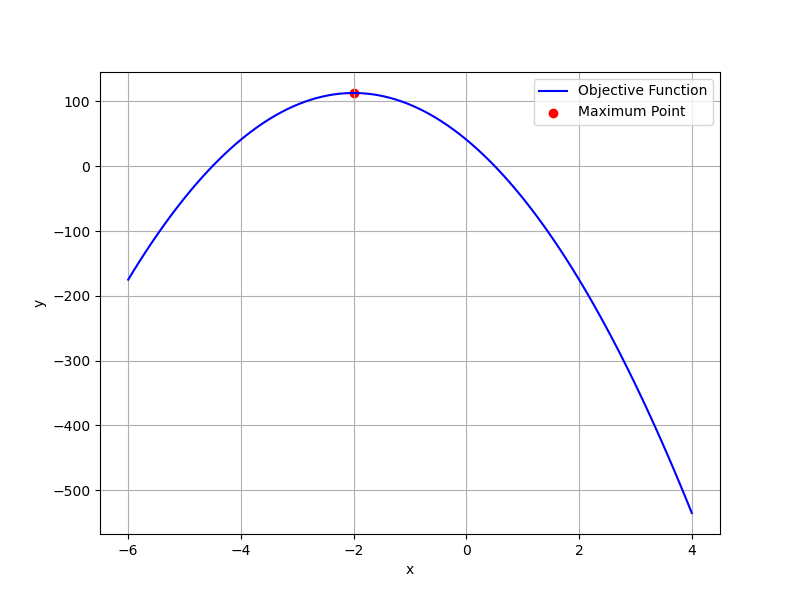
\includegraphics[width=1\linewidth]{figs/fig.png}
   \caption{Maximum Value of Objective Function}
   \label{stemplot}
\end{figure}
\end{document}
